% Options for packages loaded elsewhere
% Options for packages loaded elsewhere
\PassOptionsToPackage{unicode}{hyperref}
\PassOptionsToPackage{hyphens}{url}
\PassOptionsToPackage{dvipsnames,svgnames,x11names}{xcolor}
%
\documentclass[
  letterpaper,
  DIV=11,
  numbers=noendperiod]{scrartcl}
\usepackage{xcolor}
\usepackage{amsmath,amssymb}
\setcounter{secnumdepth}{-\maxdimen} % remove section numbering
\usepackage{iftex}
\ifPDFTeX
  \usepackage[T1]{fontenc}
  \usepackage[utf8]{inputenc}
  \usepackage{textcomp} % provide euro and other symbols
\else % if luatex or xetex
  \usepackage{unicode-math} % this also loads fontspec
  \defaultfontfeatures{Scale=MatchLowercase}
  \defaultfontfeatures[\rmfamily]{Ligatures=TeX,Scale=1}
\fi
\usepackage{lmodern}
\ifPDFTeX\else
  % xetex/luatex font selection
\fi
% Use upquote if available, for straight quotes in verbatim environments
\IfFileExists{upquote.sty}{\usepackage{upquote}}{}
\IfFileExists{microtype.sty}{% use microtype if available
  \usepackage[]{microtype}
  \UseMicrotypeSet[protrusion]{basicmath} % disable protrusion for tt fonts
}{}
\makeatletter
\@ifundefined{KOMAClassName}{% if non-KOMA class
  \IfFileExists{parskip.sty}{%
    \usepackage{parskip}
  }{% else
    \setlength{\parindent}{0pt}
    \setlength{\parskip}{6pt plus 2pt minus 1pt}}
}{% if KOMA class
  \KOMAoptions{parskip=half}}
\makeatother
% Make \paragraph and \subparagraph free-standing
\makeatletter
\ifx\paragraph\undefined\else
  \let\oldparagraph\paragraph
  \renewcommand{\paragraph}{
    \@ifstar
      \xxxParagraphStar
      \xxxParagraphNoStar
  }
  \newcommand{\xxxParagraphStar}[1]{\oldparagraph*{#1}\mbox{}}
  \newcommand{\xxxParagraphNoStar}[1]{\oldparagraph{#1}\mbox{}}
\fi
\ifx\subparagraph\undefined\else
  \let\oldsubparagraph\subparagraph
  \renewcommand{\subparagraph}{
    \@ifstar
      \xxxSubParagraphStar
      \xxxSubParagraphNoStar
  }
  \newcommand{\xxxSubParagraphStar}[1]{\oldsubparagraph*{#1}\mbox{}}
  \newcommand{\xxxSubParagraphNoStar}[1]{\oldsubparagraph{#1}\mbox{}}
\fi
\makeatother

\usepackage{color}
\usepackage{fancyvrb}
\newcommand{\VerbBar}{|}
\newcommand{\VERB}{\Verb[commandchars=\\\{\}]}
\DefineVerbatimEnvironment{Highlighting}{Verbatim}{commandchars=\\\{\}}
% Add ',fontsize=\small' for more characters per line
\usepackage{framed}
\definecolor{shadecolor}{RGB}{241,243,245}
\newenvironment{Shaded}{\begin{snugshade}}{\end{snugshade}}
\newcommand{\AlertTok}[1]{\textcolor[rgb]{0.68,0.00,0.00}{#1}}
\newcommand{\AnnotationTok}[1]{\textcolor[rgb]{0.37,0.37,0.37}{#1}}
\newcommand{\AttributeTok}[1]{\textcolor[rgb]{0.40,0.45,0.13}{#1}}
\newcommand{\BaseNTok}[1]{\textcolor[rgb]{0.68,0.00,0.00}{#1}}
\newcommand{\BuiltInTok}[1]{\textcolor[rgb]{0.00,0.23,0.31}{#1}}
\newcommand{\CharTok}[1]{\textcolor[rgb]{0.13,0.47,0.30}{#1}}
\newcommand{\CommentTok}[1]{\textcolor[rgb]{0.37,0.37,0.37}{#1}}
\newcommand{\CommentVarTok}[1]{\textcolor[rgb]{0.37,0.37,0.37}{\textit{#1}}}
\newcommand{\ConstantTok}[1]{\textcolor[rgb]{0.56,0.35,0.01}{#1}}
\newcommand{\ControlFlowTok}[1]{\textcolor[rgb]{0.00,0.23,0.31}{\textbf{#1}}}
\newcommand{\DataTypeTok}[1]{\textcolor[rgb]{0.68,0.00,0.00}{#1}}
\newcommand{\DecValTok}[1]{\textcolor[rgb]{0.68,0.00,0.00}{#1}}
\newcommand{\DocumentationTok}[1]{\textcolor[rgb]{0.37,0.37,0.37}{\textit{#1}}}
\newcommand{\ErrorTok}[1]{\textcolor[rgb]{0.68,0.00,0.00}{#1}}
\newcommand{\ExtensionTok}[1]{\textcolor[rgb]{0.00,0.23,0.31}{#1}}
\newcommand{\FloatTok}[1]{\textcolor[rgb]{0.68,0.00,0.00}{#1}}
\newcommand{\FunctionTok}[1]{\textcolor[rgb]{0.28,0.35,0.67}{#1}}
\newcommand{\ImportTok}[1]{\textcolor[rgb]{0.00,0.46,0.62}{#1}}
\newcommand{\InformationTok}[1]{\textcolor[rgb]{0.37,0.37,0.37}{#1}}
\newcommand{\KeywordTok}[1]{\textcolor[rgb]{0.00,0.23,0.31}{\textbf{#1}}}
\newcommand{\NormalTok}[1]{\textcolor[rgb]{0.00,0.23,0.31}{#1}}
\newcommand{\OperatorTok}[1]{\textcolor[rgb]{0.37,0.37,0.37}{#1}}
\newcommand{\OtherTok}[1]{\textcolor[rgb]{0.00,0.23,0.31}{#1}}
\newcommand{\PreprocessorTok}[1]{\textcolor[rgb]{0.68,0.00,0.00}{#1}}
\newcommand{\RegionMarkerTok}[1]{\textcolor[rgb]{0.00,0.23,0.31}{#1}}
\newcommand{\SpecialCharTok}[1]{\textcolor[rgb]{0.37,0.37,0.37}{#1}}
\newcommand{\SpecialStringTok}[1]{\textcolor[rgb]{0.13,0.47,0.30}{#1}}
\newcommand{\StringTok}[1]{\textcolor[rgb]{0.13,0.47,0.30}{#1}}
\newcommand{\VariableTok}[1]{\textcolor[rgb]{0.07,0.07,0.07}{#1}}
\newcommand{\VerbatimStringTok}[1]{\textcolor[rgb]{0.13,0.47,0.30}{#1}}
\newcommand{\WarningTok}[1]{\textcolor[rgb]{0.37,0.37,0.37}{\textit{#1}}}

\usepackage{longtable,booktabs,array}
\newcounter{none} % for unnumbered tables
\usepackage{calc} % for calculating minipage widths
% Correct order of tables after \paragraph or \subparagraph
\usepackage{etoolbox}
\makeatletter
\patchcmd\longtable{\par}{\if@noskipsec\mbox{}\fi\par}{}{}
\makeatother
% Allow footnotes in longtable head/foot
\IfFileExists{footnotehyper.sty}{\usepackage{footnotehyper}}{\usepackage{footnote}}
\makesavenoteenv{longtable}
\usepackage{graphicx}
\makeatletter
\newsavebox\pandoc@box
\newcommand*\pandocbounded[1]{% scales image to fit in text height/width
  \sbox\pandoc@box{#1}%
  \Gscale@div\@tempa{\textheight}{\dimexpr\ht\pandoc@box+\dp\pandoc@box\relax}%
  \Gscale@div\@tempb{\linewidth}{\wd\pandoc@box}%
  \ifdim\@tempb\p@<\@tempa\p@\let\@tempa\@tempb\fi% select the smaller of both
  \ifdim\@tempa\p@<\p@\scalebox{\@tempa}{\usebox\pandoc@box}%
  \else\usebox{\pandoc@box}%
  \fi%
}
% Set default figure placement to htbp
\def\fps@figure{htbp}
\makeatother





\setlength{\emergencystretch}{3em} % prevent overfull lines

\providecommand{\tightlist}{%
  \setlength{\itemsep}{0pt}\setlength{\parskip}{0pt}}



 


\KOMAoption{captions}{tableheading}
\makeatletter
\@ifpackageloaded{caption}{}{\usepackage{caption}}
\AtBeginDocument{%
\ifdefined\contentsname
  \renewcommand*\contentsname{Table of contents}
\else
  \newcommand\contentsname{Table of contents}
\fi
\ifdefined\listfigurename
  \renewcommand*\listfigurename{List of Figures}
\else
  \newcommand\listfigurename{List of Figures}
\fi
\ifdefined\listtablename
  \renewcommand*\listtablename{List of Tables}
\else
  \newcommand\listtablename{List of Tables}
\fi
\ifdefined\figurename
  \renewcommand*\figurename{Figure}
\else
  \newcommand\figurename{Figure}
\fi
\ifdefined\tablename
  \renewcommand*\tablename{Table}
\else
  \newcommand\tablename{Table}
\fi
}
\@ifpackageloaded{float}{}{\usepackage{float}}
\floatstyle{ruled}
\@ifundefined{c@chapter}{\newfloat{codelisting}{h}{lop}}{\newfloat{codelisting}{h}{lop}[chapter]}
\floatname{codelisting}{Listing}
\newcommand*\listoflistings{\listof{codelisting}{List of Listings}}
\makeatother
\makeatletter
\makeatother
\makeatletter
\@ifpackageloaded{caption}{}{\usepackage{caption}}
\@ifpackageloaded{subcaption}{}{\usepackage{subcaption}}
\makeatother
\usepackage{bookmark}
\IfFileExists{xurl.sty}{\usepackage{xurl}}{} % add URL line breaks if available
\urlstyle{same}
% fallback for those not using the hyperref driver hyperxmp:
\makeatletter
\@ifundefined{xmpquote}{\newcommand{\xmpquote}[1]{#1}}{}
\makeatother
\hypersetup{
  pdftitle={Financial Dashboard},
  colorlinks=true,
  linkcolor={blue},
  filecolor={Maroon},
  citecolor={Blue},
  urlcolor={Blue},
  pdfcreator={LaTeX via pandoc}}


\title{Financial Dashboard}
\author{}
\date{}
\begin{document}
\maketitle


\subsection{S\&P Historical Performance \&
Simulation}\label{sp-historical-performance-simulation}

\begin{Shaded}
\begin{Highlighting}[]
\FunctionTok{library}\NormalTok{(tidyquant)}
\end{Highlighting}
\end{Shaded}

\begin{verbatim}
Registered S3 method overwritten by 'quantmod':
  method            from
  as.zoo.data.frame zoo 
\end{verbatim}

\begin{verbatim}
-- Attaching core tidyquant packages ----------------------- tidyquant 1.0.12 --
v PerformanceAnalytics 2.1.0      v TTR                  0.24.4
v quantmod             0.4.29     v xts                  0.14.3
-- Conflicts ------------------------------------------ tidyquant_conflicts() --
x zoo::as.Date()                 masks base::as.Date()
x zoo::as.Date.numeric()         masks base::as.Date.numeric()
x PerformanceAnalytics::legend() masks graphics::legend()
x quantmod::summary()            masks base::summary()
i Use the conflicted package (<http://conflicted.r-lib.org/>) to force all conflicts to become errors
\end{verbatim}

\begin{Shaded}
\begin{Highlighting}[]
\FunctionTok{library}\NormalTok{(ggplot2)}
\FunctionTok{library}\NormalTok{(dplyr)}
\end{Highlighting}
\end{Shaded}

\begin{verbatim}

######################### Warning from 'xts' package ##########################
#                                                                             #
# The dplyr lag() function breaks how base R's lag() function is supposed to  #
# work, which breaks lag(my_xts). Calls to lag(my_xts) that you type or       #
# source() into this session won't work correctly.                            #
#                                                                             #
# Use stats::lag() to make sure you're not using dplyr::lag(), or you can add #
# conflictRules('dplyr', exclude = 'lag') to your .Rprofile to stop           #
# dplyr from breaking base R's lag() function.                                #
#                                                                             #
# Code in packages is not affected. It's protected by R's namespace mechanism #
# Set `options(xts.warn_dplyr_breaks_lag = FALSE)` to suppress this warning.  #
#                                                                             #
###############################################################################

Attaching package: 'dplyr'

The following objects are masked from 'package:xts':

    first, last

The following objects are masked from 'package:stats':

    filter, lag

The following objects are masked from 'package:base':

    intersect, setdiff, setequal, union
\end{verbatim}

\begin{Shaded}
\begin{Highlighting}[]
\NormalTok{sp500 }\OtherTok{\textless{}{-}} \FunctionTok{tq\_get}\NormalTok{(}\StringTok{"\^{}GSPC"}\NormalTok{, }
\AttributeTok{from =} \StringTok{"1950{-}01{-}01"}\NormalTok{)}
\NormalTok{sp500}
\end{Highlighting}
\end{Shaded}

\begin{verbatim}
# A tibble: 19,310 x 8
   symbol date        open  high   low close  volume adjusted
   <chr>  <date>     <dbl> <dbl> <dbl> <dbl>   <dbl>    <dbl>
 1 ^GSPC  1950-01-03  16.7  16.7  16.7  16.7 1260000     16.7
 2 ^GSPC  1950-01-04  16.9  16.9  16.9  16.9 1890000     16.9
 3 ^GSPC  1950-01-05  16.9  16.9  16.9  16.9 2550000     16.9
 4 ^GSPC  1950-01-06  17.0  17.0  17.0  17.0 2010000     17.0
 5 ^GSPC  1950-01-09  17.1  17.1  17.1  17.1 2520000     17.1
 6 ^GSPC  1950-01-10  17.0  17.0  17.0  17.0 2160000     17.0
 7 ^GSPC  1950-01-11  17.1  17.1  17.1  17.1 2630000     17.1
 8 ^GSPC  1950-01-12  16.8  16.8  16.8  16.8 2970000     16.8
 9 ^GSPC  1950-01-13  16.7  16.7  16.7  16.7 3330000     16.7
10 ^GSPC  1950-01-16  16.7  16.7  16.7  16.7 1460000     16.7
# i 19,300 more rows
\end{verbatim}

\begin{Shaded}
\begin{Highlighting}[]
\DocumentationTok{\#\#\# Index Level Over Time }\AlertTok{\#\#\#}\DocumentationTok{ We\textquotesingle{}re using the Return formula (Rt= (Pt/Pt{-}1){-}1)}
\FunctionTok{ggplot}\NormalTok{(}\AttributeTok{data =}\NormalTok{ sp500, }\FunctionTok{aes}\NormalTok{(}\AttributeTok{x =}\NormalTok{ date, }\AttributeTok{y =}\NormalTok{ adjusted)) }\SpecialCharTok{+} \FunctionTok{geom\_line}\NormalTok{()}
\end{Highlighting}
\end{Shaded}

\pandocbounded{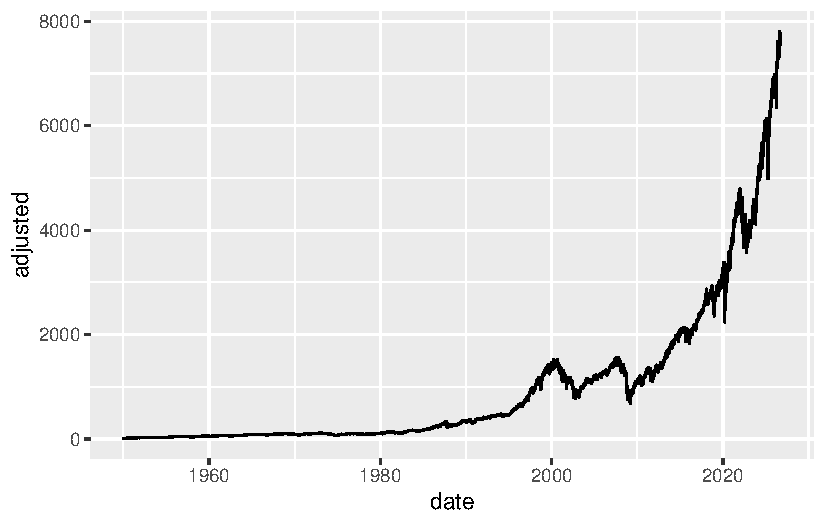
\includegraphics[keepaspectratio]{analysis_files/figure-pdf/unnamed-chunk-1-1.pdf}}

\begin{Shaded}
\begin{Highlighting}[]
\NormalTok{sp500 }\OtherTok{\textless{}{-}}\NormalTok{ sp500 }\SpecialCharTok{|\textgreater{}} 
    \FunctionTok{mutate}\NormalTok{(}
        \AttributeTok{daily\_return =}\NormalTok{ adjusted }\SpecialCharTok{/} \FunctionTok{lag}\NormalTok{(adjusted) }\SpecialCharTok{{-}}\DecValTok{1} 
\NormalTok{    )}
\FunctionTok{ggplot}\NormalTok{(}\AttributeTok{data =}\NormalTok{ sp500, }\FunctionTok{aes}\NormalTok{(}\AttributeTok{x =}\NormalTok{ date, }\AttributeTok{y =}\NormalTok{ daily\_return)) }\SpecialCharTok{+} \FunctionTok{geom\_line}\NormalTok{()}
\end{Highlighting}
\end{Shaded}

\begin{verbatim}
Warning: Removed 1 row containing missing values or values outside the scale range
(`geom_line()`).
\end{verbatim}

\pandocbounded{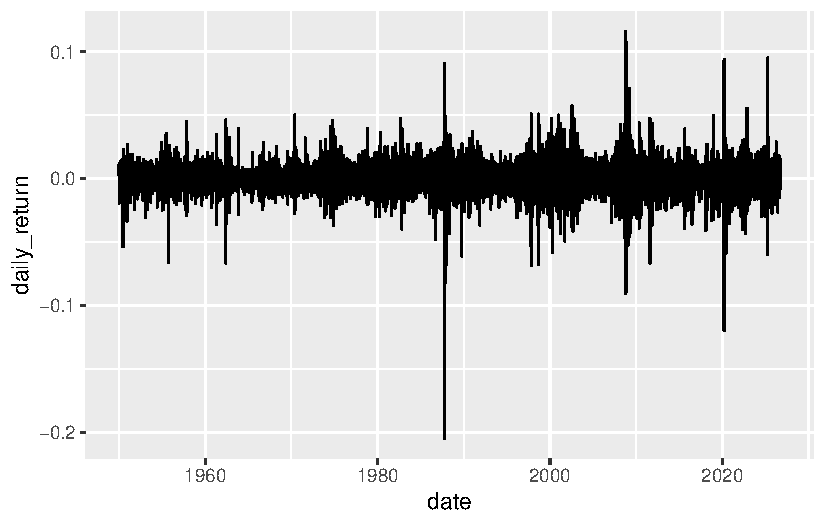
\includegraphics[keepaspectratio]{analysis_files/figure-pdf/unnamed-chunk-1-2.pdf}}

\begin{Shaded}
\begin{Highlighting}[]
\NormalTok{    sp500}
\end{Highlighting}
\end{Shaded}

\begin{verbatim}
# A tibble: 19,310 x 9
   symbol date        open  high   low close  volume adjusted daily_return
   <chr>  <date>     <dbl> <dbl> <dbl> <dbl>   <dbl>    <dbl>        <dbl>
 1 ^GSPC  1950-01-03  16.7  16.7  16.7  16.7 1260000     16.7     NA      
 2 ^GSPC  1950-01-04  16.9  16.9  16.9  16.9 1890000     16.9      0.0114 
 3 ^GSPC  1950-01-05  16.9  16.9  16.9  16.9 2550000     16.9      0.00475
 4 ^GSPC  1950-01-06  17.0  17.0  17.0  17.0 2010000     17.0      0.00295
 5 ^GSPC  1950-01-09  17.1  17.1  17.1  17.1 2520000     17.1      0.00589
 6 ^GSPC  1950-01-10  17.0  17.0  17.0  17.0 2160000     17.0     -0.00293
 7 ^GSPC  1950-01-11  17.1  17.1  17.1  17.1 2630000     17.1      0.00352
 8 ^GSPC  1950-01-12  16.8  16.8  16.8  16.8 2970000     16.8     -0.0193 
 9 ^GSPC  1950-01-13  16.7  16.7  16.7  16.7 3330000     16.7     -0.00537
10 ^GSPC  1950-01-16  16.7  16.7  16.7  16.7 1460000     16.7      0.00300
# i 19,300 more rows
\end{verbatim}

\begin{Shaded}
\begin{Highlighting}[]
\NormalTok{    annual\_returns }\OtherTok{\textless{}{-}}\NormalTok{ sp500 }\SpecialCharTok{|\textgreater{}} 
        \FunctionTok{tq\_transmute}\NormalTok{(}
            \AttributeTok{select =}\NormalTok{ adjusted,}
            \AttributeTok{mutate\_fun =}\NormalTok{ periodReturn,}
            \AttributeTok{period =} \StringTok{"yearly"}\NormalTok{,}
            \AttributeTok{type =} \StringTok{"arithmetic"}
\NormalTok{        )}
\NormalTok{        annual\_returns}
\end{Highlighting}
\end{Shaded}

\begin{verbatim}
# A tibble: 77 x 2
   date       yearly.returns
   <date>              <dbl>
 1 1950-12-29         0.226 
 2 1951-12-31         0.163 
 3 1952-12-31         0.118 
 4 1953-12-31        -0.0662
 5 1954-12-31         0.450 
 6 1955-12-30         0.264 
 7 1956-12-31         0.0262
 8 1957-12-31        -0.143 
 9 1958-12-31         0.381 
10 1959-12-31         0.0848
# i 67 more rows
\end{verbatim}

\begin{Shaded}
\begin{Highlighting}[]
        \DocumentationTok{\#\#\# Annual Returns}
        \FunctionTok{ggplot}\NormalTok{(}
            \AttributeTok{data =}\NormalTok{ annual\_returns,}
            \FunctionTok{aes}\NormalTok{(}\AttributeTok{x =}\NormalTok{ date, }\AttributeTok{y =}\NormalTok{ yearly.returns)}
\NormalTok{            ) }\SpecialCharTok{+} \FunctionTok{geom\_col}\NormalTok{() }\SpecialCharTok{+} 
                \FunctionTok{scale\_y\_continuous}\NormalTok{(}\AttributeTok{labels =}\NormalTok{ scales}\SpecialCharTok{::}\NormalTok{percent) }\SpecialCharTok{+}
                \FunctionTok{labs}\NormalTok{(}
                    \AttributeTok{title =} \StringTok{"S\&P 500 Annual Returns"}\NormalTok{,}
                    \AttributeTok{x =} \StringTok{"Year"}\NormalTok{,}
                    \AttributeTok{y =} \StringTok{"Annual Return"}
\NormalTok{                )}
\end{Highlighting}
\end{Shaded}

\pandocbounded{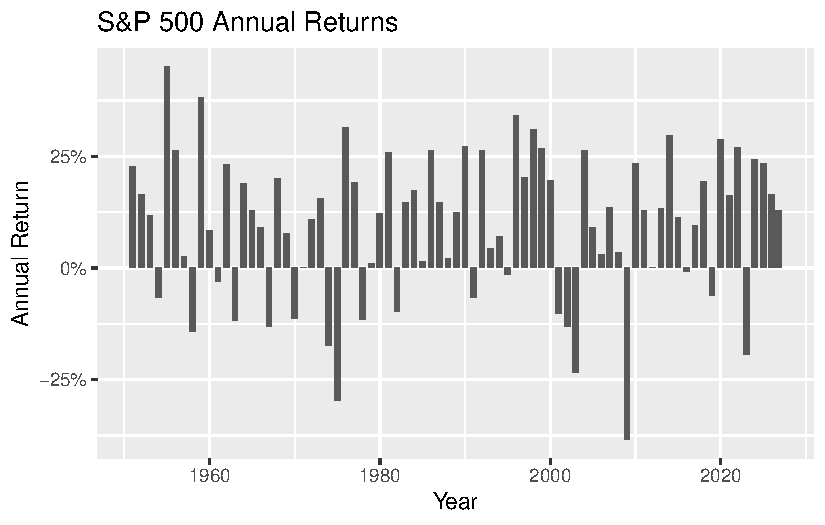
\includegraphics[keepaspectratio]{analysis_files/figure-pdf/unnamed-chunk-1-3.pdf}}

\begin{Shaded}
\begin{Highlighting}[]
                \DocumentationTok{\#\#\# Average Annnual Return, Median and Standard Deviation (Basically the volatility)}

                \FunctionTok{mean}\NormalTok{(annual\_returns}\SpecialCharTok{$}\NormalTok{yearly.returns)}
\end{Highlighting}
\end{Shaded}

\begin{verbatim}
[1] 0.09621078
\end{verbatim}

\begin{Shaded}
\begin{Highlighting}[]
                \FunctionTok{median}\NormalTok{(annual\_returns}\SpecialCharTok{$}\NormalTok{yearly.returns)}
\end{Highlighting}
\end{Shaded}

\begin{verbatim}
[1] 0.1240084
\end{verbatim}

\begin{Shaded}
\begin{Highlighting}[]
                \FunctionTok{sd}\NormalTok{(annual\_returns}\SpecialCharTok{$}\NormalTok{yearly.returns)}
\end{Highlighting}
\end{Shaded}

\begin{verbatim}
[1] 0.1642754
\end{verbatim}

\begin{Shaded}
\begin{Highlighting}[]
\DocumentationTok{\#\#\# The distribution of annual returns}

\FunctionTok{ggplot}\NormalTok{(}
    \AttributeTok{data =}\NormalTok{ annual\_returns, }
    \FunctionTok{aes}\NormalTok{(}\AttributeTok{x =}\NormalTok{ yearly.returns)}
\NormalTok{)}\SpecialCharTok{+} \FunctionTok{geom\_histogram}\NormalTok{() }\SpecialCharTok{+}
    \FunctionTok{scale\_x\_continuous}\NormalTok{(}\AttributeTok{labels =}\NormalTok{ scales}\SpecialCharTok{::}\NormalTok{percent) }\SpecialCharTok{+} 
    \FunctionTok{labs}\NormalTok{(}\AttributeTok{title =} \StringTok{"Distribution of the S\&P 500 Annual Returns"}\NormalTok{,}
    \AttributeTok{x =} \StringTok{"Annual Return"}\NormalTok{,}
    \AttributeTok{y =} \StringTok{"Number of Years"}\NormalTok{)}
\end{Highlighting}
\end{Shaded}

\begin{verbatim}
`stat_bin()` using `bins = 30`. Pick better value `binwidth`.
\end{verbatim}

\pandocbounded{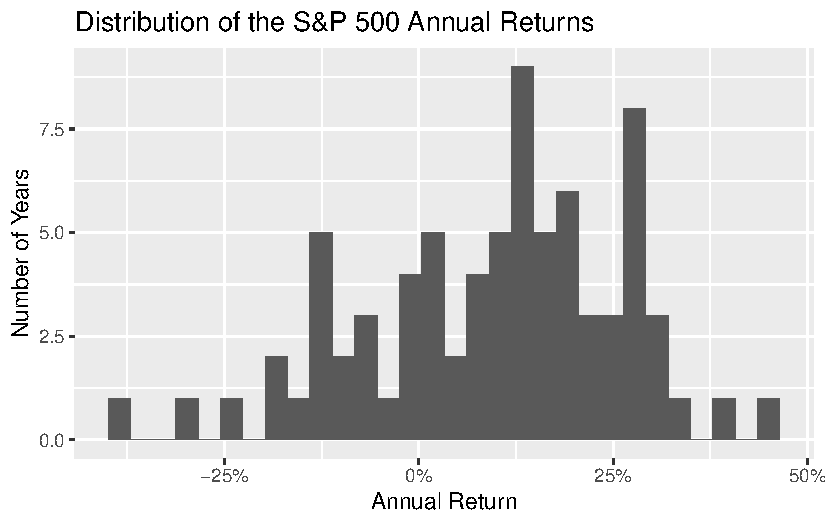
\includegraphics[keepaspectratio]{analysis_files/figure-pdf/unnamed-chunk-1-4.pdf}}

\begin{Shaded}
\begin{Highlighting}[]
\DocumentationTok{\#\#\# What percentage of years in our dataset had a negative S\&P 500 return?}
\DocumentationTok{\#\# Below is a smart way to calculate that using the mean and conditional}
\FunctionTok{mean}\NormalTok{(annual\_returns}\SpecialCharTok{$}\NormalTok{yearly.returns }\SpecialCharTok{\textless{}} \DecValTok{0}\NormalTok{)}
\end{Highlighting}
\end{Shaded}

\begin{verbatim}
[1] 0.2597403
\end{verbatim}

\begin{Shaded}
\begin{Highlighting}[]
\DocumentationTok{\#\#\# Getting the actual number of negative years}
\NormalTok{annual\_returns}\SpecialCharTok{$}\NormalTok{yearly.returns }\SpecialCharTok{\textless{}} \DecValTok{0}
\end{Highlighting}
\end{Shaded}

\begin{verbatim}
 [1] FALSE FALSE FALSE  TRUE FALSE FALSE FALSE  TRUE FALSE FALSE  TRUE FALSE
[13]  TRUE FALSE FALSE FALSE  TRUE FALSE FALSE  TRUE FALSE FALSE FALSE  TRUE
[25]  TRUE FALSE FALSE  TRUE FALSE FALSE FALSE  TRUE FALSE FALSE FALSE FALSE
[37] FALSE FALSE FALSE FALSE  TRUE FALSE FALSE FALSE  TRUE FALSE FALSE FALSE
[49] FALSE FALSE  TRUE  TRUE  TRUE FALSE FALSE FALSE FALSE FALSE  TRUE FALSE
[61] FALSE  TRUE FALSE FALSE FALSE  TRUE FALSE FALSE  TRUE FALSE FALSE FALSE
[73]  TRUE FALSE FALSE FALSE FALSE
\end{verbatim}

\begin{Shaded}
\begin{Highlighting}[]
\FunctionTok{sum}\NormalTok{(annual\_returns}\SpecialCharTok{$}\NormalTok{yearly.returns }\SpecialCharTok{\textless{}} \DecValTok{0}\NormalTok{)}
\end{Highlighting}
\end{Shaded}

\begin{verbatim}
[1] 20
\end{verbatim}

\begin{Shaded}
\begin{Highlighting}[]
\DocumentationTok{\#\#\# Calculating the Geometric Average Annual Return (Media Geometrica)}
\FunctionTok{prod}\NormalTok{(}\DecValTok{1} \SpecialCharTok{+}\NormalTok{ annual\_returns}\SpecialCharTok{$}\NormalTok{yearly.returns)}\SpecialCharTok{\^{}}\NormalTok{(}\DecValTok{1} \SpecialCharTok{/} \FunctionTok{nrow}\NormalTok{(annual\_returns)) }\SpecialCharTok{{-}} \DecValTok{1}
\end{Highlighting}
\end{Shaded}

\begin{verbatim}
[1] 0.08299042
\end{verbatim}

\begin{Shaded}
\begin{Highlighting}[]
\DocumentationTok{\#\#\# 9.61\% is the arithmetic average of individual annual returns}
\DocumentationTok{\#\#\# 8.29\% is the constant compounded annual rate equivalent to the historical sequence in our dataset}

\DocumentationTok{\#\#\# Mathematical Representation of Variation of Returns}

\NormalTok{return\_stats }\OtherTok{\textless{}{-}}\NormalTok{ annual\_returns }\SpecialCharTok{|\textgreater{}} 
    \FunctionTok{summarize}\NormalTok{(}
        \AttributeTok{mean\_return =} \FunctionTok{mean}\NormalTok{(yearly.returns),}
        \AttributeTok{median\_return =} \FunctionTok{median}\NormalTok{(yearly.returns),}
        \AttributeTok{sd\_return =} \FunctionTok{sd}\NormalTok{(yearly.returns),}
        \AttributeTok{min\_return =} \FunctionTok{min}\NormalTok{(yearly.returns),}
        \AttributeTok{max\_returns =} \FunctionTok{max}\NormalTok{(yearly.returns)}
\NormalTok{    )}

\NormalTok{    return\_stats}
\end{Highlighting}
\end{Shaded}

\begin{verbatim}
# A tibble: 1 x 5
  mean_return median_return sd_return min_return max_returns
        <dbl>         <dbl>     <dbl>      <dbl>       <dbl>
1      0.0962         0.124     0.164     -0.385       0.450
\end{verbatim}

\begin{Shaded}
\begin{Highlighting}[]
\DocumentationTok{\#\#\# THE NORMAL DISTRIBUTION}

\FunctionTok{rnorm}\NormalTok{(}
    \AttributeTok{n=}\DecValTok{1}\NormalTok{,}
    \AttributeTok{mean =}\NormalTok{ return\_stats}\SpecialCharTok{$}\NormalTok{mean\_return,}
    \AttributeTok{sd =}\NormalTok{ return\_stats}\SpecialCharTok{$}\NormalTok{sd\_return}
\NormalTok{)}
\end{Highlighting}
\end{Shaded}

\begin{verbatim}
[1] -0.1243975
\end{verbatim}

\begin{Shaded}
\begin{Highlighting}[]
\DocumentationTok{\#\#\#If you want it in \%}
\NormalTok{scales}\SpecialCharTok{::}\FunctionTok{percent}\NormalTok{(}
    \FunctionTok{rnorm}\NormalTok{(}
    \AttributeTok{n=}\DecValTok{1}\NormalTok{,}
    \AttributeTok{mean =}\NormalTok{ return\_stats}\SpecialCharTok{$}\NormalTok{mean\_return,}
    \AttributeTok{sd =}\NormalTok{ return\_stats}\SpecialCharTok{$}\NormalTok{sd\_return}
\NormalTok{)}
\NormalTok{)}
\end{Highlighting}
\end{Shaded}

\begin{verbatim}
[1] "38%"
\end{verbatim}

\begin{Shaded}
\begin{Highlighting}[]
\DocumentationTok{\#\#\# Going from one random year to a sequence of hypothetical future years.}

\NormalTok{simulated\_returns }\OtherTok{\textless{}{-}} \FunctionTok{rnorm}\NormalTok{(}
    \AttributeTok{n=}\DecValTok{30}\NormalTok{,}
    \AttributeTok{mean =}\NormalTok{ return\_stats}\SpecialCharTok{$}\NormalTok{mean\_return,}
    \AttributeTok{sd =}\NormalTok{ return\_stats}\SpecialCharTok{$}\NormalTok{sd\_return}
\NormalTok{)}
\DocumentationTok{\#\#\# a possible 30 year path.}

\DocumentationTok{\#\#\#Investing $10k once. Results in 30 years.}

\NormalTok{initial\_wealth }\OtherTok{\textless{}{-}} \DecValTok{10000}
\NormalTok{wealth\_path }\OtherTok{\textless{}{-}}\NormalTok{ initial\_wealth }\SpecialCharTok{*} \FunctionTok{cumprod}\NormalTok{(}\DecValTok{1} \SpecialCharTok{+}\NormalTok{ simulated\_returns)}

\NormalTok{wealth\_path}
\end{Highlighting}
\end{Shaded}

\begin{verbatim}
 [1]  9885.286 11345.403  9963.857  8770.963  8176.527  9012.253 12036.002
 [8] 13604.844 16630.175 19079.389 16270.570 22366.559 21247.814 26561.499
[15] 30610.444 23533.238 24723.340 24526.350 23934.835 23785.908 26466.124
[22] 28934.141 40080.930 37928.113 31146.063 24246.495 28345.524 32526.559
[29] 35364.779 30220.802
\end{verbatim}

\begin{Shaded}
\begin{Highlighting}[]
\NormalTok{simulation }\OtherTok{\textless{}{-}} \FunctionTok{data.frame}\NormalTok{(}\AttributeTok{year =} \DecValTok{1}\SpecialCharTok{:}\DecValTok{30}\NormalTok{,}
\AttributeTok{wealth =}\NormalTok{ wealth\_path)}

\NormalTok{simulation}
\end{Highlighting}
\end{Shaded}

\begin{verbatim}
   year    wealth
1     1  9885.286
2     2 11345.403
3     3  9963.857
4     4  8770.963
5     5  8176.527
6     6  9012.253
7     7 12036.002
8     8 13604.844
9     9 16630.175
10   10 19079.389
11   11 16270.570
12   12 22366.559
13   13 21247.814
14   14 26561.499
15   15 30610.444
16   16 23533.238
17   17 24723.340
18   18 24526.350
19   19 23934.835
20   20 23785.908
21   21 26466.124
22   22 28934.141
23   23 40080.930
24   24 37928.113
25   25 31146.063
26   26 24246.495
27   27 28345.524
28   28 32526.559
29   29 35364.779
30   30 30220.802
\end{verbatim}

\begin{Shaded}
\begin{Highlighting}[]
\FunctionTok{ggplot}\NormalTok{(}
    \AttributeTok{data =}\NormalTok{ simulation,}
    \FunctionTok{aes}\NormalTok{(}\AttributeTok{x =}\NormalTok{ year, }\AttributeTok{y =}\NormalTok{ wealth)) }\SpecialCharTok{+} 
        \FunctionTok{geom\_line}\NormalTok{() }\SpecialCharTok{+} 
        \FunctionTok{labs}\NormalTok{(}
            \AttributeTok{title =} \StringTok{"One Simulated 30{-}Year Investment Path"}\NormalTok{,}
            \AttributeTok{x =} \StringTok{"Year"}\NormalTok{,}
            \AttributeTok{y =} \StringTok{"Portfolio Value"}
\NormalTok{        )}
\end{Highlighting}
\end{Shaded}

\pandocbounded{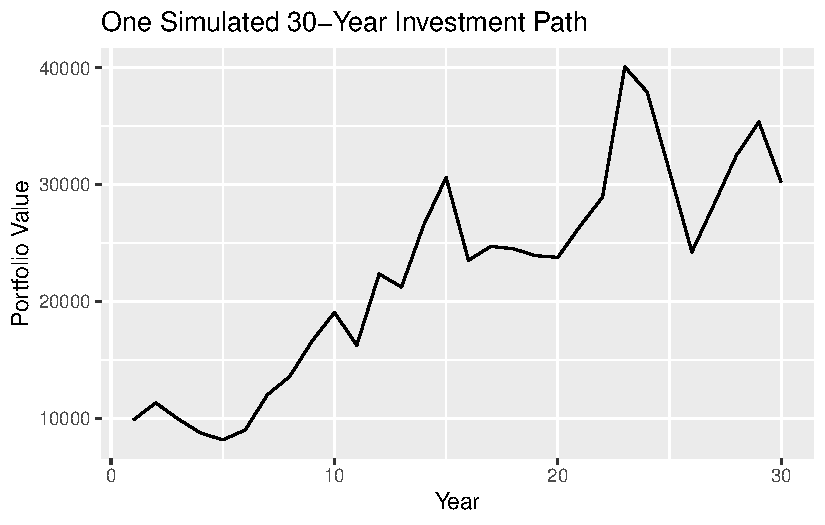
\includegraphics[keepaspectratio]{analysis_files/figure-pdf/unnamed-chunk-1-5.pdf}}

\begin{Shaded}
\begin{Highlighting}[]
\DocumentationTok{\#\#\# Let\textquotesingle{}s make it start from year 0 (10K)}

\NormalTok{simulation }\OtherTok{\textless{}{-}} \FunctionTok{data.frame}\NormalTok{(}
    \AttributeTok{year =} \DecValTok{0}\SpecialCharTok{:}\DecValTok{30}\NormalTok{,}
    \AttributeTok{wealth =} \FunctionTok{c}\NormalTok{(initial\_wealth, wealth\_path))}

\DocumentationTok{\#\#\# Then run the same plot as before.}

\DocumentationTok{\#\#\# Let\textquotesingle{}s run 3 simulated paths}

\NormalTok{simulated\_returns\_3 }\OtherTok{\textless{}{-}} \FunctionTok{matrix}\NormalTok{(}
    \FunctionTok{rnorm}\NormalTok{(}
        \AttributeTok{n =} \DecValTok{30} \SpecialCharTok{*} \DecValTok{3}\NormalTok{,}
        \AttributeTok{mean =}\NormalTok{ return\_stats}\SpecialCharTok{$}\NormalTok{mean\_return,}
        \AttributeTok{sd =}\NormalTok{ return\_stats}\SpecialCharTok{$}\NormalTok{sd\_return}
\NormalTok{    ),}
    \AttributeTok{nrow =} \DecValTok{30}\NormalTok{,}
    \AttributeTok{ncol =} \DecValTok{3}
\NormalTok{)}

\NormalTok{simulated\_returns\_3}
\end{Highlighting}
\end{Shaded}

\begin{verbatim}
              [,1]         [,2]         [,3]
 [1,] -0.378019968  0.164320556 -0.090296852
 [2,] -0.171824501  0.358316655  0.131332971
 [3,]  0.019782134  0.344339174  0.158561173
 [4,]  0.378859277 -0.194282987  0.098085768
 [5,] -0.037906178 -0.200285777  0.366690059
 [6,]  0.054170523  0.204838477  0.311150130
 [7,]  0.317579488 -0.044761849  0.158560277
 [8,]  0.292561010 -0.015669027 -0.121514180
 [9,]  0.003441871 -0.044772018  0.220557961
[10,] -0.232951544  0.221933795 -0.042264140
[11,]  0.343618573  0.240788628  0.281601168
[12,] -0.006671470 -0.003870685  0.125352329
[13,]  0.006739781 -0.080072091 -0.240393228
[14,]  0.166190779  0.061284026  0.007695918
[15,]  0.172030811  0.005395766  0.097362632
[16,] -0.022843703  0.169302545 -0.096208558
[17,]  0.251641432  0.033995915  0.445057505
[18,]  0.081139934  0.269281320 -0.081817195
[19,]  0.145838794 -0.027073165 -0.074239401
[20,] -0.064723805  0.226611067  0.114172031
[21,]  0.179789315  0.093323151  0.196134776
[22,] -0.016275891  0.252809124  0.148812673
[23,]  0.138258073  0.194811317  0.244762931
[24,] -0.005668859  0.083738157  0.116663109
[25,]  0.168778177  0.244905888  0.088316613
[26,]  0.069426362  0.009155231  0.066610838
[27,]  0.151786428  0.136630346  0.071978867
[28,]  0.002822890  0.226048438  0.066901091
[29,]  0.056523401 -0.067835366  0.191524174
[30,] -0.045030403  0.052559467  0.109500808
\end{verbatim}

\begin{Shaded}
\begin{Highlighting}[]
\DocumentationTok{\#\#\# Converting those returns into wealth paths}

\NormalTok{wealth\_paths\_3 }\OtherTok{\textless{}{-}} \FunctionTok{apply}\NormalTok{(}
\NormalTok{    simulated\_returns\_3,}
    \DecValTok{2}\NormalTok{,}
    \ControlFlowTok{function}\NormalTok{(x) initial\_wealth }\SpecialCharTok{*} \FunctionTok{cumprod}\NormalTok{(}\DecValTok{1} \SpecialCharTok{+}\NormalTok{ x)}
\NormalTok{)}
\NormalTok{wealth\_paths\_3}
\end{Highlighting}
\end{Shaded}

\begin{verbatim}
           [,1]      [,2]       [,3]
 [1,]  6219.800  11643.21   9097.031
 [2,]  5151.086  15815.16  10291.772
 [3,]  5252.986  21260.94  11923.647
 [4,]  7243.128  17130.30  13093.187
 [5,]  6968.569  13699.34  17894.329
 [6,]  7346.060  16505.50  23462.151
 [7,]  9679.018  15766.68  27182.317
 [8,] 12510.721  15519.63  23879.280
 [9,] 12553.781  14824.79  29146.045
[10,]  9629.358  18114.91  27914.212
[11,] 12938.185  22476.77  35774.887
[12,] 12851.868  22389.77  40259.353
[13,] 12938.487  20596.98  30581.277
[14,] 15088.744  21859.24  30816.628
[15,] 17684.473  21977.19  33817.016
[16,] 17280.494  25697.98  30563.530
[17,] 21628.983  26571.61  44166.058
[18,] 23383.957  33726.85  40552.515
[19,] 26794.245  32813.76  37541.920
[20,] 25060.019  40249.72  41828.158
[21,] 29565.543  44005.95  50032.114
[22,] 29084.337  55131.05  57477.527
[23,] 33105.482  65871.20  71545.894
[24,] 32917.812  71387.14  79892.661
[25,] 38473.620  88870.27  86948.510
[26,] 41144.703  89683.89  92740.223
[27,] 47389.911 101937.44  99415.560
[28,] 47523.687 124980.23 106066.569
[29,] 50209.888 116502.15 126380.881
[30,] 47948.916 122625.45 140219.690
\end{verbatim}

\begin{Shaded}
\begin{Highlighting}[]
\DocumentationTok{\#\#\# Visualizing these 3 simulations}
\NormalTok{simulation\_3 }\OtherTok{\textless{}{-}} \FunctionTok{data.frame}\NormalTok{(}
    \AttributeTok{year =} \DecValTok{0}\SpecialCharTok{:}\DecValTok{30}\NormalTok{,}
    \AttributeTok{path\_1 =} \FunctionTok{c}\NormalTok{(initial\_wealth, wealth\_paths\_3[, }\DecValTok{1}\NormalTok{]),}
    \AttributeTok{path\_2 =} \FunctionTok{c}\NormalTok{(initial\_wealth, wealth\_paths\_3[, }\DecValTok{2}\NormalTok{]),}
    \AttributeTok{path\_3 =} \FunctionTok{c}\NormalTok{(initial\_wealth, wealth\_paths\_3[, }\DecValTok{3}\NormalTok{])}
\NormalTok{)}

\NormalTok{simulation\_3}
\end{Highlighting}
\end{Shaded}

\begin{verbatim}
   year    path_1    path_2     path_3
1     0 10000.000  10000.00  10000.000
2     1  6219.800  11643.21   9097.031
3     2  5151.086  15815.16  10291.772
4     3  5252.986  21260.94  11923.647
5     4  7243.128  17130.30  13093.187
6     5  6968.569  13699.34  17894.329
7     6  7346.060  16505.50  23462.151
8     7  9679.018  15766.68  27182.317
9     8 12510.721  15519.63  23879.280
10    9 12553.781  14824.79  29146.045
11   10  9629.358  18114.91  27914.212
12   11 12938.185  22476.77  35774.887
13   12 12851.868  22389.77  40259.353
14   13 12938.487  20596.98  30581.277
15   14 15088.744  21859.24  30816.628
16   15 17684.473  21977.19  33817.016
17   16 17280.494  25697.98  30563.530
18   17 21628.983  26571.61  44166.058
19   18 23383.957  33726.85  40552.515
20   19 26794.245  32813.76  37541.920
21   20 25060.019  40249.72  41828.158
22   21 29565.543  44005.95  50032.114
23   22 29084.337  55131.05  57477.527
24   23 33105.482  65871.20  71545.894
25   24 32917.812  71387.14  79892.661
26   25 38473.620  88870.27  86948.510
27   26 41144.703  89683.89  92740.223
28   27 47389.911 101937.44  99415.560
29   28 47523.687 124980.23 106066.569
30   29 50209.888 116502.15 126380.881
31   30 47948.916 122625.45 140219.690
\end{verbatim}

\begin{Shaded}
\begin{Highlighting}[]
\FunctionTok{ggplot}\NormalTok{(}\AttributeTok{data =}\NormalTok{ simulation\_3,}
\FunctionTok{aes}\NormalTok{(}\AttributeTok{x =}\NormalTok{ year)) }\SpecialCharTok{+} 
    \FunctionTok{geom\_line}\NormalTok{(}\FunctionTok{aes}\NormalTok{(}\AttributeTok{y =}\NormalTok{ path\_1)) }\SpecialCharTok{+} 
    \FunctionTok{geom\_line}\NormalTok{(}\FunctionTok{aes}\NormalTok{(}\AttributeTok{y =}\NormalTok{ path\_2)) }\SpecialCharTok{+}
    \FunctionTok{geom\_line}\NormalTok{(}\FunctionTok{aes}\NormalTok{(}\AttributeTok{y =}\NormalTok{ path\_3)) }\SpecialCharTok{+} 
    \FunctionTok{labs}\NormalTok{(}
        \AttributeTok{title =} \StringTok{"Three Simulated 30{-}Year Investment Paths"}\NormalTok{,}
            \AttributeTok{x =} \StringTok{"Year"}\NormalTok{,}
            \AttributeTok{y =} \StringTok{"Portfolio Value"}\NormalTok{,}
\NormalTok{    )}
\end{Highlighting}
\end{Shaded}

\pandocbounded{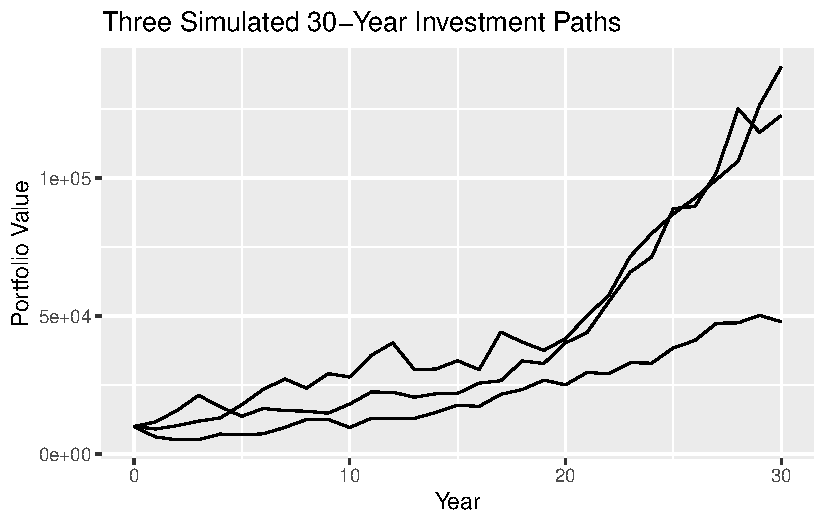
\includegraphics[keepaspectratio]{analysis_files/figure-pdf/unnamed-chunk-1-6.pdf}}

\begin{Shaded}
\begin{Highlighting}[]
    \DocumentationTok{\#\#\# Transforming the dataset from Wide format to Long format. }

    \FunctionTok{library}\NormalTok{(tidyr)}
\NormalTok{    simulation\_3\_long }\OtherTok{\textless{}{-}}\NormalTok{ simulation\_3 }\SpecialCharTok{|\textgreater{}}
        \FunctionTok{pivot\_longer}\NormalTok{(}
            \AttributeTok{cols =} \FunctionTok{starts\_with}\NormalTok{(}\StringTok{"path\_"}\NormalTok{),}
            \AttributeTok{names\_to =} \StringTok{"path"}\NormalTok{,}
            \AttributeTok{values\_to =} \StringTok{"wealth"}
\NormalTok{        )}
\NormalTok{        simulation\_3\_long}
\end{Highlighting}
\end{Shaded}

\begin{verbatim}
# A tibble: 93 x 3
    year path   wealth
   <int> <chr>   <dbl>
 1     0 path_1 10000 
 2     0 path_2 10000 
 3     0 path_3 10000 
 4     1 path_1  6220.
 5     1 path_2 11643.
 6     1 path_3  9097.
 7     2 path_1  5151.
 8     2 path_2 15815.
 9     2 path_3 10292.
10     3 path_1  5253.
# i 83 more rows
\end{verbatim}

\begin{Shaded}
\begin{Highlighting}[]
        \FunctionTok{ggplot}\NormalTok{(}
            \AttributeTok{data =}\NormalTok{ simulation\_3\_long,}
            \FunctionTok{aes}\NormalTok{(}
                \AttributeTok{x =}\NormalTok{ year,}
                \AttributeTok{y =}\NormalTok{ wealth,}
                \AttributeTok{group =}\NormalTok{ path}
\NormalTok{            )}
\NormalTok{        ) }\SpecialCharTok{+}
            \FunctionTok{geom\_line}\NormalTok{() }\SpecialCharTok{+}
            \FunctionTok{labs}\NormalTok{(}
                \AttributeTok{title =} \StringTok{"Three Simulated 30 Year Investment Paths"}\NormalTok{,}
                \AttributeTok{x =} \StringTok{"Year"}\NormalTok{,}
                \AttributeTok{y =} \StringTok{"Portfolio Value"}
\NormalTok{            )}
\end{Highlighting}
\end{Shaded}

\pandocbounded{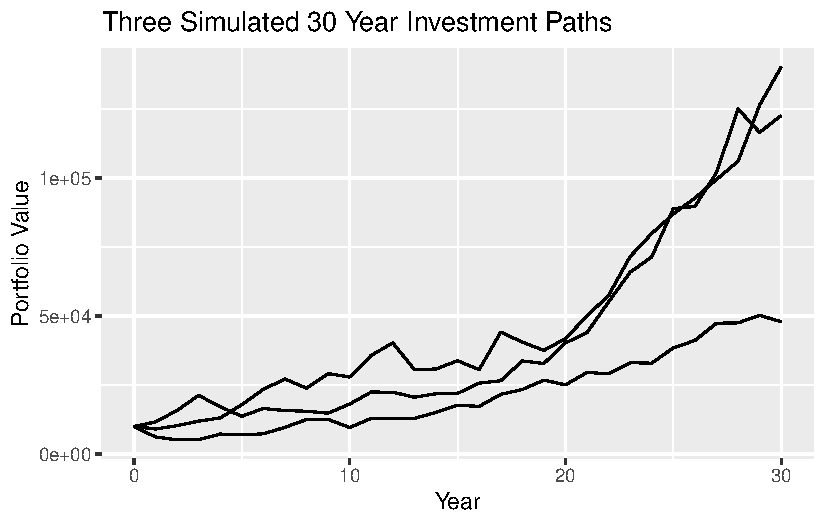
\includegraphics[keepaspectratio]{analysis_files/figure-pdf/unnamed-chunk-1-7.pdf}}

\begin{Shaded}
\begin{Highlighting}[]
\DocumentationTok{\#\#\# group = path connects observations belonging to the same path together. }

\DocumentationTok{\#\#\# MONTECARLO SIMULATION: 1000 POSSIBLE 30 YEAR FUTURES}

\NormalTok{n\_years }\OtherTok{\textless{}{-}} \DecValTok{30}
\NormalTok{n\_simulations }\OtherTok{\textless{}{-}} \DecValTok{1000}

\FunctionTok{set.seed}\NormalTok{(}\DecValTok{123}\NormalTok{) }\DocumentationTok{\#\#\# if you rerun the code with seed 123 (or whatever number), you get the same sequence again.}

\NormalTok{simulated\_returns\_1000 }\OtherTok{\textless{}{-}} \FunctionTok{matrix}\NormalTok{(}
    \FunctionTok{rnorm}\NormalTok{(}
        \AttributeTok{n =}\NormalTok{ n\_years }\SpecialCharTok{*}\NormalTok{ n\_simulations,}
        \AttributeTok{mean =}\NormalTok{ return\_stats}\SpecialCharTok{$}\NormalTok{mean\_return,}
        \AttributeTok{sd =}\NormalTok{ return\_stats}\SpecialCharTok{$}\NormalTok{sd\_return}
\NormalTok{    ),}
    \AttributeTok{nrow =}\NormalTok{ n\_years,}
    \AttributeTok{ncol =}\NormalTok{ n\_simulations}
\NormalTok{)}

\FunctionTok{dim}\NormalTok{(simulated\_returns\_1000)}
\end{Highlighting}
\end{Shaded}

\begin{verbatim}
[1]   30 1000
\end{verbatim}

\begin{Shaded}
\begin{Highlighting}[]
\DocumentationTok{\#\#\# Compunding Formula to each column}

\NormalTok{wealth\_paths\_1000 }\OtherTok{\textless{}{-}} \FunctionTok{apply}\NormalTok{(}
\NormalTok{    simulated\_returns\_1000,}
    \DecValTok{2}\NormalTok{,}
    \ControlFlowTok{function}\NormalTok{(x) initial\_wealth }\SpecialCharTok{*} \FunctionTok{cumprod}\NormalTok{(}\DecValTok{1} \SpecialCharTok{+}\NormalTok{ x)}
\NormalTok{)}
\FunctionTok{dim}\NormalTok{(wealth\_paths\_1000)}
\end{Highlighting}
\end{Shaded}

\begin{verbatim}
[1]   30 1000
\end{verbatim}

\begin{Shaded}
\begin{Highlighting}[]
\DocumentationTok{\#\#\# Let\textquotesingle{}s see the final row (where the investor ended up after the 30 years in each of the 1000 scenarios)}

\NormalTok{ending\_wealth }\OtherTok{\textless{}{-}}\NormalTok{ wealth\_paths\_1000[n\_years, ]  }\DocumentationTok{\#\#\# We had set up n\_years = 30. So row 30.}
\NormalTok{ending\_wealth}
\end{Highlighting}
\end{Shaded}

\begin{verbatim}
   [1]   92228.330  279263.332  135705.638   78581.384   43463.099  241176.610
   [7]  125797.021   81956.474  141592.431  537299.893  150070.399   58872.636
  [13]  139850.412   35347.844  117571.145  391184.108  137632.668  233014.260
  [19]  158578.444   43360.886   43708.484   71867.253   36506.600  162379.829
  [25]  385088.593  176565.368  146553.075   28016.085  319239.346  292523.170
  [31]  444977.151   45166.461   56090.804  180588.032  196937.653  193404.461
  [37]   78056.517  156276.979   79970.300  129277.635   35671.368  192991.512
  [43]  109018.327  156377.021   44155.051  121060.259  149338.488  134242.306
  [49]  310453.781  132524.670  204068.200  265001.545   96344.300  141432.307
  [55]  220698.174  140124.686   75199.251   59043.690  180206.688  163500.070
  [61]  169874.690   58663.047  274114.689  198167.933   82420.525  188838.714
  [67]  127343.136  233221.175  112605.219   12861.608  174421.948   24524.829
  [73]   44756.564  319541.814   49471.250   31928.829  119050.383  155047.879
  [79]  111685.732  172064.064   13181.262  220002.571  119627.362  507446.144
  [85]   53512.665  453318.328  145214.958  131248.941  112019.342   14683.522
  [91]   32853.100  173016.988  206893.991  124730.436   96262.990  236231.128
  [97]   81634.557   30111.473  528028.645  439595.880  111571.457   49275.269
 [103]  138962.966   45123.778   35909.351   60569.648  109119.440  565756.478
 [109]  105896.839   39926.207   99425.657  279506.722  197860.261   92993.402
 [115]   53788.402  420512.856   44168.342   52789.995  152335.121  456808.487
 [121]   52009.768  140080.747   75546.945  174650.539   49190.763   35678.467
 [127]   38828.695  107904.276  338084.188   92412.765  188100.536  540697.887
 [133]  168370.432   61578.303   57798.539   41857.282  114386.239  145173.728
 [139]   44691.293  217093.063   68535.396  101116.742  181954.659   88703.633
 [145]   47176.628  227502.357   69315.103  417591.703   21296.126   59585.149
 [151]  490498.845  111076.413  129965.656   57728.735  268578.184  111316.784
 [157]  104582.291   94328.945  168870.778   36854.232   83850.378   68431.895
 [163]   92844.647  166637.098   51446.361   96502.330   62998.097   63445.933
 [169]  120877.166  436942.890   83190.333   74516.415  232277.440   67795.786
 [175]  134116.601  130690.278  147827.591   48672.089  155521.276   66703.350
 [181]  131393.239  391811.314  104158.974  113013.820  180331.296   90765.576
 [187]   80969.206   73099.224  376596.741  112701.208   96836.545  317104.768
 [193]   51697.157  443984.239   63985.439  115758.530   79075.034  261398.307
 [199]  201687.840  218144.243  152914.329  135899.599  145695.647   31210.665
 [205]   23185.793   19884.354  104931.547  169743.754  131863.858  335283.079
 [211]   23030.692  120277.171   20839.593  119650.176  127622.093  726555.922
 [217]  452145.179  229494.059  201198.233  103069.477   47843.515  126903.739
 [223]   89503.425   31478.441  148234.634   27474.381   52506.613  111019.316
 [229]   73228.039  514206.836   41309.474   84529.985  152443.773  139769.036
 [235]  276516.116   93599.755   42777.352  136943.659   52105.146  129257.804
 [241]  208194.239  568660.356  163693.057  428652.050   39743.562   61976.885
 [247]  260746.340  119410.547  237795.343  140805.004   24847.424   39094.039
 [253]  242576.645   64550.111  150726.576   99334.149  305286.015   24233.455
 [259]  215534.359  160053.354  311020.380  202797.933  135093.587    6463.477
 [265]   43171.818  224948.524   38624.194  164818.153   27825.798  154977.642
 [271]   79590.181   51390.050  269920.651   56434.765  430087.034  151384.079
 [277]  807463.505  221022.990   80060.740  325872.853  147277.598   89931.312
 [283]   50042.979  266075.429   60486.092  320785.322  175620.316   40151.608
 [289]  426540.766   43785.083  165761.680   89295.559  114162.450  386474.595
 [295]  186206.997  155995.270   40814.973   39098.266   42049.549   34018.007
 [301]  227177.002  156541.727   79880.948   89447.927   76157.416   89956.377
 [307]   79851.929   81574.820  118790.548   39832.007   78761.849   71747.154
 [313]   58494.184  193229.728  106291.919  277034.602   75907.479  401510.945
 [319]   99080.285   14316.339  152032.832  178618.977   70431.596   76596.017
 [325]   65585.163   56879.171  141935.833   20678.857   67624.894   91505.237
 [331]  160958.843   41133.155  160747.233   87953.385  229244.150  129831.499
 [337]   87008.715   24267.484  307573.304   70378.696  408648.200  373411.087
 [343]  358416.919  129725.508   46866.067  307510.470  168578.436  128815.389
 [349]  173128.592   30733.096  106501.018  297467.466  454121.315  102316.996
 [355]   55880.132   87879.686   58657.357   83748.874  102352.259  167489.254
 [361]  392642.499  104473.653   97505.030  120681.386   15876.207  167933.464
 [367]   71245.039  420799.806   89866.055   79604.433  119525.788   76653.211
 [373]  767447.220  162446.972  184692.380   98166.135  220169.120  286392.409
 [379]  168030.160   84792.700   41212.351  315222.994   70016.504  262826.098
 [385]  102697.959  293789.277   51475.343  247710.313   35960.744   36535.353
 [391]   74140.462   66218.280   95526.225   45303.944  425039.158   53702.928
 [397]   85484.332  217598.295  177424.137  228383.906  177964.731   99375.128
 [403]   43729.524   86600.494   42941.553   36480.461 1532381.831  168672.787
 [409]   18864.837   86495.681  224412.645   16032.772   53005.947   48664.938
 [415]  146008.886   78758.379   21612.047  160872.964   67291.138  122288.667
 [421]  119750.972  288991.948   56128.769  249096.795   41708.149  137757.688
 [427]   49281.039   87326.879  124304.052   25526.295  568202.295   35638.838
 [433]   22678.015   88844.227  267001.060  489401.843  249923.447   91109.345
 [439]  361846.417  152747.398   74833.476   65324.387   57514.061  148444.254
 [445]  136579.661  207386.174  408218.527   28200.616  139340.043  145838.118
 [451]   80062.011  277510.693  115675.324   90524.642   57829.727  123522.296
 [457]  121614.298   79527.464   45954.581  217923.708   58419.806  101603.898
 [463]  323931.710  356126.438  313700.144   22006.960  164145.285  270430.839
 [469]   92964.656  398957.553  127030.585   78193.547   55096.409  105356.807
 [475]  110821.554  100049.668  266234.939   73396.151  127512.240  211404.560
 [481]  121305.404  146047.480  141312.388  185236.525   45915.233  186473.631
 [487]  137480.441  130331.398   10617.349  174446.163   73352.065  100033.999
 [493]  166375.663   64323.356  124348.634  162005.710  128775.808  392008.581
 [499]   67609.677  164832.149   88998.267   94647.923   73910.150  169540.524
 [505]   47371.963  278696.638  789478.841  117275.455  169576.814  193776.719
 [511]  358741.418   87058.975  159561.436   66001.526   53285.826  441997.121
 [517]  238694.555   63671.936  307062.470   66801.422  154843.295   62271.156
 [523]   43811.339   36977.264  108843.209  205687.509   13958.281  300042.768
 [529]   77513.935  111461.192   52775.814   64156.063  117291.614  207576.281
 [535]   34418.992  150739.772   81739.834  138795.665  252115.729   85835.993
 [541]  310134.674   42308.699   31701.532   21507.109   30843.771  110582.733
 [547]  193042.168   20559.305  122194.879  375207.580  116576.306  123629.553
 [553]  106169.010  133977.666  103769.138  115288.766   65509.761   66471.604
 [559]   65361.699   65766.235  213734.749   43179.383   72920.880   76505.139
 [565]   15439.388  108685.642  301190.630   33296.824   68896.099  127851.606
 [571]   91865.632  208090.216  239183.642   49231.041   67312.730   87331.613
 [577]  261059.905  253493.548   40101.673   14265.549   58746.770   70705.855
 [583]  318064.194  104401.950  123144.694  115225.614   96715.788   61776.719
 [589]  239976.798  129439.100  237407.291  283851.321  150593.858   33725.741
 [595]  138060.869   46160.695  100796.703  104810.010  131416.564  156632.669
 [601]  134157.435   47495.170  152086.288   76012.718  246287.923  170706.945
 [607]  101226.178  100243.965   41570.477   64271.883   59008.225  299181.043
 [613]   48254.118  312864.664   64956.003   41678.570   63376.080  172957.302
 [619]   57314.017  173984.128   79608.468  330180.797   51262.195   11709.452
 [625]   32869.830  118676.825   70679.510  293797.962  101140.670  541925.853
 [631]  123932.331  152589.880  140638.159   79094.703  116596.758   63627.474
 [637]  958777.186   25289.130   81500.907  241167.799   64490.028   33701.686
 [643]   46400.040  262094.198   48422.273   74827.075  234995.646   94398.924
 [649]   67911.326  276142.270  117586.605   21343.887   86151.704  121031.840
 [655]  263646.031   59361.250   24428.565   39865.338  356419.775  258719.786
 [661]   54943.087  180409.630  119969.277   36015.622   32917.801   61211.556
 [667]   32503.751   94385.590   94693.640  407558.059   12734.181   83050.225
 [673]   43759.529   44512.963   84160.490   79075.840  108182.761  129560.613
 [679]  568019.520  421307.092  246420.618  178496.740  310226.140   89113.559
 [685]   43703.206   82114.457    9260.974   78406.461  268271.325   49103.922
 [691]  275877.458  461936.743   81681.647  268152.891  209515.815   16511.760
 [697]   35807.836  119450.335   80243.078  136571.652   55586.287  228599.960
 [703]  436451.488  110656.427   89964.251   23195.271  111787.081   38983.812
 [709]  123397.113   23329.757   92065.656   90543.289  364025.968 1008190.688
 [715]   57330.923  208163.574  186671.386   36431.382  155368.465  356026.071
 [721]  178739.368  176378.629   53400.626  245009.549  448725.572  107663.260
 [727]   92534.172   55968.755  204371.216   71698.945   90152.739   25668.179
 [733]   69831.567   30428.171  104504.676   30611.935  427163.614  134975.128
 [739]   66741.293   41729.156   69533.943  147197.898   40379.649   67202.904
 [745]  251940.984  298072.116  136079.713   29260.214  169988.843   91278.611
 [751]  415241.515   95623.577  348412.004  129644.073  118219.442  116551.871
 [757]   53574.982   16037.344  147457.731   57756.917  107734.088  217886.403
 [763]   41281.944   75546.908   61140.819  341943.861  156393.007   25106.096
 [769]  210317.020   14927.725  160157.589  148061.136   89344.713  174754.970
 [775]  164568.619  141958.872   94859.598  340291.622  461443.187   86999.501
 [781]  161843.666   83220.786   70588.341  176955.350   30170.358  352656.218
 [787]   84051.508  232518.364  160339.921  155140.844   42413.020  244476.912
 [793]  117343.438  127822.331   78350.406  511384.771  231796.192  276721.209
 [799]   30600.170  246732.447  431642.683  139629.031   52919.257   56781.496
 [805]  261193.869  127064.985  160979.991   39918.907   37350.437   44198.840
 [811]  132703.638   27258.934  175354.699  227861.370  121109.616   32825.420
 [817]   99924.662  103855.846   12358.066  461149.841   41560.622  569853.537
 [823]   44055.686  140937.736  153806.452   89000.498  339228.455   58761.657
 [829]   24496.240  127082.292   53159.369   43230.883   53614.582  246533.231
 [835]  149842.629  151210.760  460647.933  241626.535  164977.513  130989.333
 [841]   71102.454   47006.284  356508.120  213033.128   62093.552   77298.611
 [847]   38611.538  156177.297   38904.061  521801.998   52791.743  139113.443
 [853]   54709.382   55073.828   41034.034   43844.787  121248.941  102628.482
 [859]   71410.719  105683.302  117387.150   97713.064  107496.758   34733.375
 [865]   78544.460  141754.606  100407.026   71653.130  106618.414  184816.669
 [871]   54264.650   93662.929   47656.590   30161.702   73163.977   28362.595
 [877]  670018.682   68239.179  119715.388   25384.445  127103.705  127676.080
 [883]   22767.438  165284.175  132742.248  103409.847   49108.033   10392.938
 [889]  142370.340  577900.565  108931.851  171984.712   64420.136   80297.237
 [895]   81040.030  164963.470  423582.212   91412.640  309387.199  161230.250
 [901]   41102.079   36190.921  155670.457  137056.017   31517.342  297440.453
 [907]  117723.132   99271.494  142186.303  161904.862   38296.123   67329.359
 [913]   93489.476   71168.310  169501.795   50520.252  177049.807   70430.708
 [919]  102466.930   76481.436  228005.473  170083.818  174431.231  239578.549
 [925]   65091.520  115882.623  384249.230   60393.860   98079.251  165592.765
 [931]  414167.184   47637.828  191203.495  342557.664  446694.549   42765.051
 [937]   93190.535   42962.020  690332.561  169596.147   66235.915  272777.299
 [943]  136034.631   57004.654  290628.671  144484.528   44563.179  140596.669
 [949]  156544.760  165464.326   39509.234   27984.343  130996.570   81632.165
 [955]   61234.410  149887.332   53516.677   81260.993  191552.102   59097.417
 [961]  111091.005  148076.555   94625.322  327583.771  237731.730   62855.962
 [967]  104910.394  146973.418   12582.682  173763.225  229095.171   68816.243
 [973]   40209.183   33260.015  200868.934  426141.214  107779.524  293928.858
 [979]   40991.997  244310.628   25596.793  170737.852  136923.903   19736.717
 [985]  405584.022  120638.659  149924.439  143638.682  112358.558  289402.085
 [991]  182279.291  118383.683  457166.810  293051.450   69064.452   55887.598
 [997]  214021.949  494253.067  516002.186   54553.527
\end{verbatim}

\begin{Shaded}
\begin{Highlighting}[]
\FunctionTok{length}\NormalTok{(ending\_wealth)}
\end{Highlighting}
\end{Shaded}

\begin{verbatim}
[1] 1000
\end{verbatim}

\begin{Shaded}
\begin{Highlighting}[]
\FunctionTok{summary}\NormalTok{(ending\_wealth)}
\end{Highlighting}
\end{Shaded}

\begin{verbatim}
   Min. 1st Qu.  Median    Mean 3rd Qu.   lth After 30 Years",
        x = "Ending Portfolio Value",
        y = "Number of Simulations"
    )
\end{verbatim}

\begin{verbatim}
`stat_bin()` using `bins = 30`. Pick better value `binwidth`.
\end{verbatim}

\pandocbounded{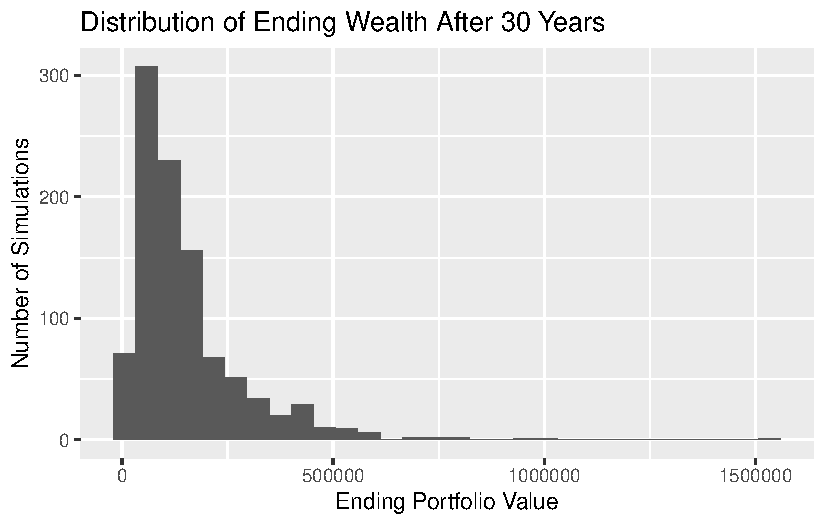
\includegraphics[keepaspectratio]{analysis_files/figure-pdf/unnamed-chunk-1-8.pdf}}

\begin{Shaded}
\begin{Highlighting}[]
    \DocumentationTok{\#\#\# Percentiles}
    \FunctionTok{quantile}\NormalTok{(}
\NormalTok{        ending\_wealth,}
        \AttributeTok{probs =} \FunctionTok{c}\NormalTok{(}\FloatTok{0.10}\NormalTok{, }\FloatTok{0.50}\NormalTok{, }\FloatTok{0.90}\NormalTok{)}
\NormalTok{    )}
\end{Highlighting}
\end{Shaded}

\begin{verbatim}
      10%       50%       90% 
 38622.93 111628.59 313852.43 
\end{verbatim}

\begin{Shaded}
\begin{Highlighting}[]
\NormalTok{median\_path }\OtherTok{\textless{}{-}} \FunctionTok{apply}\NormalTok{(}
\NormalTok{    wealth\_paths\_1000,}
    \DecValTok{1}\NormalTok{,}
\NormalTok{    median}
\NormalTok{)    }
\NormalTok{median\_path}
\end{Highlighting}
\end{Shaded}

\begin{verbatim}
 [1]  10959.61  12014.55  13096.08  14194.21  15352.52  16592.32  17745.50
 [8]  19265.18  20815.53  22565.89  24474.18  26278.00  28785.65  31618.13
[15]  33743.16  35898.85  39636.10  42733.95  47326.07  50517.81  53983.88
[22]  59891.83  64630.54  70086.76  73964.30  80837.74  87771.25  96854.24
[29] 106116.50 111628.59
\end{verbatim}

\begin{Shaded}
\begin{Highlighting}[]
\NormalTok{lower\_path }\OtherTok{\textless{}{-}} \FunctionTok{apply}\NormalTok{(}
\NormalTok{    wealth\_paths\_1000,}
    \DecValTok{1}\NormalTok{,}
\NormalTok{    quantile,}
    \AttributeTok{probs =} \FloatTok{0.90}
\NormalTok{)}
\NormalTok{lower\_path}
\end{Highlighting}
\end{Shaded}

\begin{verbatim}
 [1]  13098.94  15615.55  17825.02  20471.81  23258.57  26453.57  29868.91
 [8]  33788.97  37914.40  42797.51  48558.92  53031.78  59816.60  64829.55
[15]  70965.82  77492.68  85202.81  94039.01 103024.45 114990.59 128076.99
[22] 140278.50 160651.11 182671.71 196503.99 213736.84 241392.68 260140.56
[29] 284220.55 313852.43
\end{verbatim}

\begin{Shaded}
\begin{Highlighting}[]
\NormalTok{upper\_path }\OtherTok{\textless{}{-}} \FunctionTok{apply}\NormalTok{(}
\NormalTok{    wealth\_paths\_1000,}
    \DecValTok{1}\NormalTok{,}
\NormalTok{    quantile,}
    \AttributeTok{probs =} \FloatTok{0.10}
\NormalTok{)}
\NormalTok{upper\_path}
\end{Highlighting}
\end{Shaded}

\begin{verbatim}
 [1]  8971.313  8840.484  9009.503  8887.985  9165.170  9758.577 10118.703
 [8] 10640.051 11189.062 11748.443 12671.651 12963.068 13738.091 14328.323
[15] 15124.539 15864.469 17374.689 18099.402 19343.186 20725.162 22903.838
[22] 24271.505 24437.851 26701.157 28781.817 29591.533 31276.445 32126.272
[29] 34746.108 38622.928
\end{verbatim}

\begin{Shaded}
\begin{Highlighting}[]
\DocumentationTok{\#\#\# Putting median\_path, lower\_path and upper\_path in one data frame}

\NormalTok{percentile\_paths }\OtherTok{\textless{}{-}} \FunctionTok{data.frame}\NormalTok{(}
    \AttributeTok{year =} \DecValTok{1}\SpecialCharTok{:}\NormalTok{n\_years,}
    \AttributeTok{lower =}\NormalTok{ lower\_path,}
    \AttributeTok{median =}\NormalTok{ median\_path,}
    \AttributeTok{upper =}\NormalTok{ upper\_path}
\NormalTok{)}

\NormalTok{percentile\_paths}
\end{Highlighting}
\end{Shaded}

\begin{verbatim}
   year     lower    median     upper
1     1  13098.94  10959.61  8971.313
2     2  15615.55  12014.55  8840.484
3     3  17825.02  13096.08  9009.503
4     4  20471.81  14194.21  8887.985
5     5  23258.57  15352.52  9165.170
6     6  26453.57  16592.32  9758.577
7     7  29868.91  17745.50 10118.703
8     8  33788.97  19265.18 10640.051
9     9  37914.40  20815.53 11189.062
10   10  42797.51  22565.89 11748.443
11   11  48558.92  24474.18 12671.651
12   12  53031.78  26278.00 12963.068
13   13  59816.60  28785.65 13738.091
14   14  64829.55  31618.13 14328.323
15   15  70965.82  33743.16 15124.539
16   16  77492.68  35898.85 15864.469
17   17  85202.81  39636.10 17374.689
18   18  94039.01  42733.95 18099.402
19   19 103024.45  47326.07 19343.186
20   20 114990.59  50517.81 20725.162
21   21 128076.99  53983.88 22903.838
22   22 140278.50  59891.83 24271.505
23   23 160651.11  64630.54 24437.851
24   24 182671.71  70086.76 26701.157
25   25 196503.99  73964.30 28781.817
26   26 213736.84  80837.74 29591.533
27   27 241392.68  87771.25 31276.445
28   28 260140.56  96854.24 32126.272
29   29 284220.55 106116.50 34746.108
30   30 313852.43 111628.59 38622.928
\end{verbatim}

\begin{Shaded}
\begin{Highlighting}[]
\DocumentationTok{\#\#\#}

\FunctionTok{ggplot}\NormalTok{(}
    \AttributeTok{data =}\NormalTok{ percentile\_paths,}
    \FunctionTok{aes}\NormalTok{(}\AttributeTok{x =}\NormalTok{ year)}
\NormalTok{) }\SpecialCharTok{+}
    \FunctionTok{geom\_ribbon}\NormalTok{(}
        \FunctionTok{aes}\NormalTok{(}\AttributeTok{ymin =}\NormalTok{ lower, }\AttributeTok{ymax =}\NormalTok{ upper),}
        \AttributeTok{alpha =} \FloatTok{0.3}
\NormalTok{    ) }\SpecialCharTok{+} 
        \FunctionTok{geom\_line}\NormalTok{(}
            \FunctionTok{aes}\NormalTok{(}\AttributeTok{y =}\NormalTok{ median)}
\NormalTok{        ) }\SpecialCharTok{+} 
            \FunctionTok{labs}\NormalTok{(}
                \AttributeTok{title =} \StringTok{"Montecarlo Simulation of Portfolio Wealth"}\NormalTok{,}
                \AttributeTok{x =} \StringTok{"Year"}\NormalTok{,}
                \AttributeTok{y =} \StringTok{"Portfolio Value"}
\NormalTok{            )}
\end{Highlighting}
\end{Shaded}

\pandocbounded{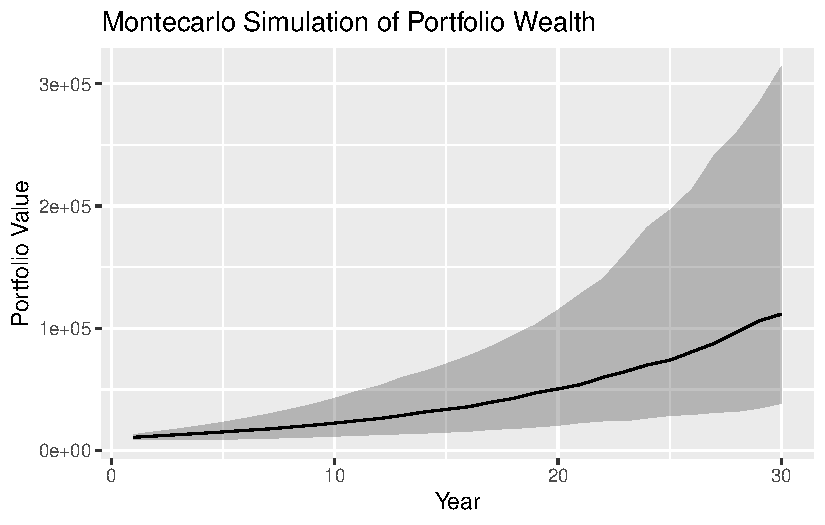
\includegraphics[keepaspectratio]{analysis_files/figure-pdf/unnamed-chunk-1-9.pdf}}

\begin{verbatim}
 ) + 
        labs(
            title = "Montecarlo Simulation of Portfolio Wealth",
            x = "Year",
            y = "Portfolio Value"
        )
\end{verbatim}

```

\pandocbounded{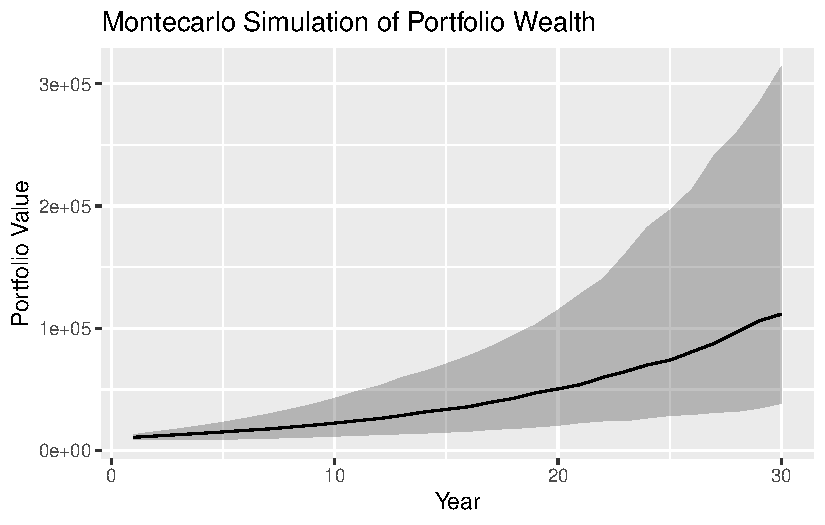
\includegraphics[keepaspectratio]{analysis_files/figure-pdf/unnamed-chunk-1-9.pdf}}




\end{document}
